\documentclass[14pt]{extbook}
\usepackage{multicol, enumerate, enumitem, hyperref, color, soul, setspace, parskip, fancyhdr} %General Packages
\usepackage{amssymb, amsthm, amsmath, bbm, latexsym, units, mathtools} %Math Packages
\everymath{\displaystyle} %All math in Display Style
% Packages with additional options
\usepackage[headsep=0.5cm,headheight=12pt, left=1 in,right= 1 in,top= 1 in,bottom= 1 in]{geometry}
\usepackage[usenames,dvipsnames]{xcolor}
\usepackage{dashrule}  % Package to use the command below to create lines between items
\newcommand{\litem}[1]{\item#1\hspace*{-1cm}\rule{\textwidth}{0.4pt}}
\pagestyle{fancy}
\lhead{Progress Quiz 1}
\chead{}
\rhead{Version B}
\lfoot{2654-6976}
\cfoot{}
\rfoot{Fall 2020}
\begin{document}

\begin{enumerate}
\litem{
First, find the equation of the line containing the two points below. Then, write the equation as $ y=mx+b $ and choose the intervals that contain $m$ and $b$.\[ (-4, 7) \text{ and } (-8, -2) \]\begin{enumerate}[label=\Alph*.]
\item \( m \in [2.25, 3.25] \hspace*{3mm} b \in [16, 21] \)
\item \( m \in [2.25, 3.25] \hspace*{3mm} b \in [7, 12] \)
\item \( m \in [2.25, 3.25] \hspace*{3mm} b \in [3, 8] \)
\item \( m \in [2.25, 3.25] \hspace*{3mm} b \in [-16, -10] \)
\item \( m \in [-3.25, -0.25] \hspace*{3mm} b \in [-25, -18] \)

\end{enumerate} }
\litem{
Find the equation of the line described below. Write the linear equation as $ y=mx+b $ and choose the intervals that contain $m$ and $b$.\[ \text{Perpendicular to } 8 x - 3 y = 10 \text{ and passing through the point } (2, 10). \]\begin{enumerate}[label=\Alph*.]
\item \( m \in [-1.3, 0.1] \hspace*{3mm} b \in [10.47, 11.43] \)
\item \( m \in [0.1, 1.8] \hspace*{3mm} b \in [8.72, 9.49] \)
\item \( m \in [-2.8, -1.2] \hspace*{3mm} b \in [10.47, 11.43] \)
\item \( m \in [-1.3, 0.1] \hspace*{3mm} b \in [-11.92, -10.38] \)
\item \( m \in [-1.3, 0.1] \hspace*{3mm} b \in [7.18, 9.04] \)

\end{enumerate} }
\litem{
Solve the equation below. Then, choose the interval that contains the solution.\[ -8(18x + 4) = -17(-3x -16) \]\begin{enumerate}[label=\Alph*.]
\item \( x \in [-1.42, -1.22] \)
\item \( x \in [1.18, 1.39] \)
\item \( x \in [2.2, 2.88] \)
\item \( x \in [-1.58, -1.44] \)
\item \( \text{There are no real solutions.} \)

\end{enumerate} }
\litem{
Solve the linear equation below. Then, choose the interval that contains the solution.\[ \frac{-8x -4}{5} - \frac{-7x + 9}{7} = \frac{-9x -7}{8} \]\begin{enumerate}[label=\Alph*.]
\item \( x \in [1.6, 2.8] \)
\item \( x \in [-1, 1.2] \)
\item \( x \in [-4.6, -0.4] \)
\item \( x \in [10.7, 11.8] \)
\item \( \text{There are no real solutions.} \)

\end{enumerate} }
\litem{
Write the equation of the line in the graph below in Standard form $Ax+By=C$. Then, choose the intervals that contain $A, B, \text{ and } C$.
\begin{center}
    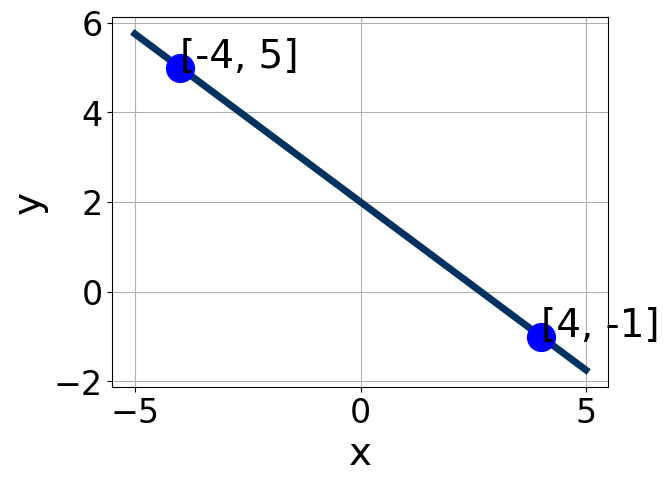
\includegraphics[width=0.5\textwidth]{../Figures/linearGraphToStandardCopyB.png}
\end{center}
\begin{enumerate}[label=\Alph*.]
\item \( A \in [-0.8, 1.2], \hspace{3mm} B \in [-1.48, -0.51], \text{ and } \hspace{3mm} C \in [-1, 3] \)
\item \( A \in [3, 10], \hspace{3mm} B \in [-6.55, -3.96], \text{ and } \hspace{3mm} C \in [4, 16] \)
\item \( A \in [-6, -3], \hspace{3mm} B \in [3.98, 5.33], \text{ and } \hspace{3mm} C \in [-11, -8] \)
\item \( A \in [-0.8, 1.2], \hspace{3mm} B \in [0.15, 2.17], \text{ and } \hspace{3mm} C \in [-5, 1] \)
\item \( A \in [3, 10], \hspace{3mm} B \in [3.98, 5.33], \text{ and } \hspace{3mm} C \in [-11, -8] \)

\end{enumerate} }
\litem{
Solve the linear equation below. Then, choose the interval that contains the solution.\[ \frac{3x -4}{7} - \frac{-6x -9}{8} = \frac{7x -5}{3} \]\begin{enumerate}[label=\Alph*.]
\item \( x \in [0.5, 2.3] \)
\item \( x \in [-3.2, -1] \)
\item \( x \in [-0.5, 1.7] \)
\item \( x \in [7.7, 9] \)
\item \( \text{There are no real solutions.} \)

\end{enumerate} }
\litem{
Write the equation of the line in the graph below in Standard form $Ax+By=C$. Then, choose the intervals that contain $A, B, \text{ and } C$.
\begin{center}
    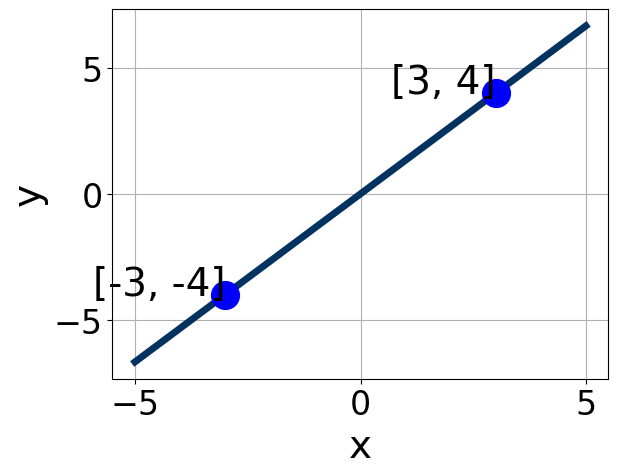
\includegraphics[width=0.5\textwidth]{../Figures/linearGraphToStandardB.png}
\end{center}
\begin{enumerate}[label=\Alph*.]
\item \( A \in [-8, -1], \hspace{3mm} B \in [-6.2, -2.6], \text{ and } \hspace{3mm} C \in [-5, 1] \)
\item \( A \in [0.8, 3.8], \hspace{3mm} B \in [-1.5, 0.8], \text{ and } \hspace{3mm} C \in [-5, 1] \)
\item \( A \in [2, 7], \hspace{3mm} B \in [-6.2, -2.6], \text{ and } \hspace{3mm} C \in [-5, 1] \)
\item \( A \in [2, 7], \hspace{3mm} B \in [3.6, 6.7], \text{ and } \hspace{3mm} C \in [-5, 1] \)
\item \( A \in [0.8, 3.8], \hspace{3mm} B \in [-0.1, 1.7], \text{ and } \hspace{3mm} C \in [-5, 1] \)

\end{enumerate} }
\litem{
First, find the equation of the line containing the two points below. Then, write the equation as $ y=mx+b $ and choose the intervals that contain $m$ and $b$.\[ (6, -7) \text{ and } (-5, -6) \]\begin{enumerate}[label=\Alph*.]
\item \( m \in [-0.19, 0.07] \hspace*{3mm} b \in [-1.93, -0.82] \)
\item \( m \in [-0.19, 0.07] \hspace*{3mm} b \in [-6.99, -6.45] \)
\item \( m \in [0.01, 0.38] \hspace*{3mm} b \in [-6.42, -5.27] \)
\item \( m \in [-0.19, 0.07] \hspace*{3mm} b \in [-13.18, -10.89] \)
\item \( m \in [-0.19, 0.07] \hspace*{3mm} b \in [5.74, 6.94] \)

\end{enumerate} }
\litem{
Solve the equation below. Then, choose the interval that contains the solution.\[ -7(9x -18) = -19(16x + 17) \]\begin{enumerate}[label=\Alph*.]
\item \( x \in [-1.18, -0.65] \)
\item \( x \in [-2.36, -1.58] \)
\item \( x \in [-0.78, -0.22] \)
\item \( x \in [0.57, 1.03] \)
\item \( \text{There are no real solutions.} \)

\end{enumerate} }
\litem{
Find the equation of the line described below. Write the linear equation as $ y=mx+b $ and choose the intervals that contain $m$ and $b$.\[ \text{Perpendicular to } 3 x - 4 y = 8 \text{ and passing through the point } (-3, 10). \]\begin{enumerate}[label=\Alph*.]
\item \( m \in [0.8, 1.72] \hspace*{3mm} b \in [13.33, 15.06] \)
\item \( m \in [-2.46, -1.21] \hspace*{3mm} b \in [12.94, 13.33] \)
\item \( m \in [-0.84, -0.59] \hspace*{3mm} b \in [4.97, 7.26] \)
\item \( m \in [-2.46, -1.21] \hspace*{3mm} b \in [4.97, 7.26] \)
\item \( m \in [-2.46, -1.21] \hspace*{3mm} b \in [-7.01, -4.86] \)

\end{enumerate} }
\end{enumerate}

\end{document}